
% Default to the notebook output style

    


% Inherit from the specified cell style.




    
\documentclass[11pt]{article}

    
    
    \usepackage[T1]{fontenc}
    % Nicer default font (+ math font) than Computer Modern for most use cases
    \usepackage{mathpazo}

    % Basic figure setup, for now with no caption control since it's done
    % automatically by Pandoc (which extracts ![](path) syntax from Markdown).
    \usepackage{graphicx}
    % We will generate all images so they have a width \maxwidth. This means
    % that they will get their normal width if they fit onto the page, but
    % are scaled down if they would overflow the margins.
    \makeatletter
    \def\maxwidth{\ifdim\Gin@nat@width>\linewidth\linewidth
    \else\Gin@nat@width\fi}
    \makeatother
    \let\Oldincludegraphics\includegraphics
    % Set max figure width to be 80% of text width, for now hardcoded.
    \renewcommand{\includegraphics}[1]{\Oldincludegraphics[width=.8\maxwidth]{#1}}
    % Ensure that by default, figures have no caption (until we provide a
    % proper Figure object with a Caption API and a way to capture that
    % in the conversion process - todo).
    \usepackage{caption}
    \DeclareCaptionLabelFormat{nolabel}{}
    \captionsetup{labelformat=nolabel}

    \usepackage{adjustbox} % Used to constrain images to a maximum size 
    \usepackage{xcolor} % Allow colors to be defined
    \usepackage{enumerate} % Needed for markdown enumerations to work
    \usepackage{geometry} % Used to adjust the document margins
    \usepackage{amsmath} % Equations
    \usepackage{amssymb} % Equations
    \usepackage{textcomp} % defines textquotesingle
    % Hack from http://tex.stackexchange.com/a/47451/13684:
    \AtBeginDocument{%
        \def\PYZsq{\textquotesingle}% Upright quotes in Pygmentized code
    }
    \usepackage{upquote} % Upright quotes for verbatim code
    \usepackage{eurosym} % defines \euro
    \usepackage[mathletters]{ucs} % Extended unicode (utf-8) support
    \usepackage[utf8x]{inputenc} % Allow utf-8 characters in the tex document
    \usepackage{fancyvrb} % verbatim replacement that allows latex
    \usepackage{grffile} % extends the file name processing of package graphics 
                         % to support a larger range 
    % The hyperref package gives us a pdf with properly built
    % internal navigation ('pdf bookmarks' for the table of contents,
    % internal cross-reference links, web links for URLs, etc.)
    \usepackage{hyperref}
    \usepackage{longtable} % longtable support required by pandoc >1.10
    \usepackage{booktabs}  % table support for pandoc > 1.12.2
    \usepackage[inline]{enumitem} % IRkernel/repr support (it uses the enumerate* environment)
    \usepackage[normalem]{ulem} % ulem is needed to support strikethroughs (\sout)
                                % normalem makes italics be italics, not underlines
    

    
    
    % Colors for the hyperref package
    \definecolor{urlcolor}{rgb}{0,.145,.698}
    \definecolor{linkcolor}{rgb}{.71,0.21,0.01}
    \definecolor{citecolor}{rgb}{.12,.54,.11}

    % ANSI colors
    \definecolor{ansi-black}{HTML}{3E424D}
    \definecolor{ansi-black-intense}{HTML}{282C36}
    \definecolor{ansi-red}{HTML}{E75C58}
    \definecolor{ansi-red-intense}{HTML}{B22B31}
    \definecolor{ansi-green}{HTML}{00A250}
    \definecolor{ansi-green-intense}{HTML}{007427}
    \definecolor{ansi-yellow}{HTML}{DDB62B}
    \definecolor{ansi-yellow-intense}{HTML}{B27D12}
    \definecolor{ansi-blue}{HTML}{208FFB}
    \definecolor{ansi-blue-intense}{HTML}{0065CA}
    \definecolor{ansi-magenta}{HTML}{D160C4}
    \definecolor{ansi-magenta-intense}{HTML}{A03196}
    \definecolor{ansi-cyan}{HTML}{60C6C8}
    \definecolor{ansi-cyan-intense}{HTML}{258F8F}
    \definecolor{ansi-white}{HTML}{C5C1B4}
    \definecolor{ansi-white-intense}{HTML}{A1A6B2}

    % commands and environments needed by pandoc snippets
    % extracted from the output of `pandoc -s`
    \providecommand{\tightlist}{%
      \setlength{\itemsep}{0pt}\setlength{\parskip}{0pt}}
    \DefineVerbatimEnvironment{Highlighting}{Verbatim}{commandchars=\\\{\}}
    % Add ',fontsize=\small' for more characters per line
    \newenvironment{Shaded}{}{}
    \newcommand{\KeywordTok}[1]{\textcolor[rgb]{0.00,0.44,0.13}{\textbf{{#1}}}}
    \newcommand{\DataTypeTok}[1]{\textcolor[rgb]{0.56,0.13,0.00}{{#1}}}
    \newcommand{\DecValTok}[1]{\textcolor[rgb]{0.25,0.63,0.44}{{#1}}}
    \newcommand{\BaseNTok}[1]{\textcolor[rgb]{0.25,0.63,0.44}{{#1}}}
    \newcommand{\FloatTok}[1]{\textcolor[rgb]{0.25,0.63,0.44}{{#1}}}
    \newcommand{\CharTok}[1]{\textcolor[rgb]{0.25,0.44,0.63}{{#1}}}
    \newcommand{\StringTok}[1]{\textcolor[rgb]{0.25,0.44,0.63}{{#1}}}
    \newcommand{\CommentTok}[1]{\textcolor[rgb]{0.38,0.63,0.69}{\textit{{#1}}}}
    \newcommand{\OtherTok}[1]{\textcolor[rgb]{0.00,0.44,0.13}{{#1}}}
    \newcommand{\AlertTok}[1]{\textcolor[rgb]{1.00,0.00,0.00}{\textbf{{#1}}}}
    \newcommand{\FunctionTok}[1]{\textcolor[rgb]{0.02,0.16,0.49}{{#1}}}
    \newcommand{\RegionMarkerTok}[1]{{#1}}
    \newcommand{\ErrorTok}[1]{\textcolor[rgb]{1.00,0.00,0.00}{\textbf{{#1}}}}
    \newcommand{\NormalTok}[1]{{#1}}
    
    % Additional commands for more recent versions of Pandoc
    \newcommand{\ConstantTok}[1]{\textcolor[rgb]{0.53,0.00,0.00}{{#1}}}
    \newcommand{\SpecialCharTok}[1]{\textcolor[rgb]{0.25,0.44,0.63}{{#1}}}
    \newcommand{\VerbatimStringTok}[1]{\textcolor[rgb]{0.25,0.44,0.63}{{#1}}}
    \newcommand{\SpecialStringTok}[1]{\textcolor[rgb]{0.73,0.40,0.53}{{#1}}}
    \newcommand{\ImportTok}[1]{{#1}}
    \newcommand{\DocumentationTok}[1]{\textcolor[rgb]{0.73,0.13,0.13}{\textit{{#1}}}}
    \newcommand{\AnnotationTok}[1]{\textcolor[rgb]{0.38,0.63,0.69}{\textbf{\textit{{#1}}}}}
    \newcommand{\CommentVarTok}[1]{\textcolor[rgb]{0.38,0.63,0.69}{\textbf{\textit{{#1}}}}}
    \newcommand{\VariableTok}[1]{\textcolor[rgb]{0.10,0.09,0.49}{{#1}}}
    \newcommand{\ControlFlowTok}[1]{\textcolor[rgb]{0.00,0.44,0.13}{\textbf{{#1}}}}
    \newcommand{\OperatorTok}[1]{\textcolor[rgb]{0.40,0.40,0.40}{{#1}}}
    \newcommand{\BuiltInTok}[1]{{#1}}
    \newcommand{\ExtensionTok}[1]{{#1}}
    \newcommand{\PreprocessorTok}[1]{\textcolor[rgb]{0.74,0.48,0.00}{{#1}}}
    \newcommand{\AttributeTok}[1]{\textcolor[rgb]{0.49,0.56,0.16}{{#1}}}
    \newcommand{\InformationTok}[1]{\textcolor[rgb]{0.38,0.63,0.69}{\textbf{\textit{{#1}}}}}
    \newcommand{\WarningTok}[1]{\textcolor[rgb]{0.38,0.63,0.69}{\textbf{\textit{{#1}}}}}
    
    
    % Define a nice break command that doesn't care if a line doesn't already
    % exist.
    \def\br{\hspace*{\fill} \\* }
    % Math Jax compatability definitions
    \def\gt{>}
    \def\lt{<}
    % Document parameters
    \title{quality\_and\_reliability.notes}
    
    
    

    % Pygments definitions
    
\makeatletter
\def\PY@reset{\let\PY@it=\relax \let\PY@bf=\relax%
    \let\PY@ul=\relax \let\PY@tc=\relax%
    \let\PY@bc=\relax \let\PY@ff=\relax}
\def\PY@tok#1{\csname PY@tok@#1\endcsname}
\def\PY@toks#1+{\ifx\relax#1\empty\else%
    \PY@tok{#1}\expandafter\PY@toks\fi}
\def\PY@do#1{\PY@bc{\PY@tc{\PY@ul{%
    \PY@it{\PY@bf{\PY@ff{#1}}}}}}}
\def\PY#1#2{\PY@reset\PY@toks#1+\relax+\PY@do{#2}}

\expandafter\def\csname PY@tok@w\endcsname{\def\PY@tc##1{\textcolor[rgb]{0.73,0.73,0.73}{##1}}}
\expandafter\def\csname PY@tok@c\endcsname{\let\PY@it=\textit\def\PY@tc##1{\textcolor[rgb]{0.25,0.50,0.50}{##1}}}
\expandafter\def\csname PY@tok@cp\endcsname{\def\PY@tc##1{\textcolor[rgb]{0.74,0.48,0.00}{##1}}}
\expandafter\def\csname PY@tok@k\endcsname{\let\PY@bf=\textbf\def\PY@tc##1{\textcolor[rgb]{0.00,0.50,0.00}{##1}}}
\expandafter\def\csname PY@tok@kp\endcsname{\def\PY@tc##1{\textcolor[rgb]{0.00,0.50,0.00}{##1}}}
\expandafter\def\csname PY@tok@kt\endcsname{\def\PY@tc##1{\textcolor[rgb]{0.69,0.00,0.25}{##1}}}
\expandafter\def\csname PY@tok@o\endcsname{\def\PY@tc##1{\textcolor[rgb]{0.40,0.40,0.40}{##1}}}
\expandafter\def\csname PY@tok@ow\endcsname{\let\PY@bf=\textbf\def\PY@tc##1{\textcolor[rgb]{0.67,0.13,1.00}{##1}}}
\expandafter\def\csname PY@tok@nb\endcsname{\def\PY@tc##1{\textcolor[rgb]{0.00,0.50,0.00}{##1}}}
\expandafter\def\csname PY@tok@nf\endcsname{\def\PY@tc##1{\textcolor[rgb]{0.00,0.00,1.00}{##1}}}
\expandafter\def\csname PY@tok@nc\endcsname{\let\PY@bf=\textbf\def\PY@tc##1{\textcolor[rgb]{0.00,0.00,1.00}{##1}}}
\expandafter\def\csname PY@tok@nn\endcsname{\let\PY@bf=\textbf\def\PY@tc##1{\textcolor[rgb]{0.00,0.00,1.00}{##1}}}
\expandafter\def\csname PY@tok@ne\endcsname{\let\PY@bf=\textbf\def\PY@tc##1{\textcolor[rgb]{0.82,0.25,0.23}{##1}}}
\expandafter\def\csname PY@tok@nv\endcsname{\def\PY@tc##1{\textcolor[rgb]{0.10,0.09,0.49}{##1}}}
\expandafter\def\csname PY@tok@no\endcsname{\def\PY@tc##1{\textcolor[rgb]{0.53,0.00,0.00}{##1}}}
\expandafter\def\csname PY@tok@nl\endcsname{\def\PY@tc##1{\textcolor[rgb]{0.63,0.63,0.00}{##1}}}
\expandafter\def\csname PY@tok@ni\endcsname{\let\PY@bf=\textbf\def\PY@tc##1{\textcolor[rgb]{0.60,0.60,0.60}{##1}}}
\expandafter\def\csname PY@tok@na\endcsname{\def\PY@tc##1{\textcolor[rgb]{0.49,0.56,0.16}{##1}}}
\expandafter\def\csname PY@tok@nt\endcsname{\let\PY@bf=\textbf\def\PY@tc##1{\textcolor[rgb]{0.00,0.50,0.00}{##1}}}
\expandafter\def\csname PY@tok@nd\endcsname{\def\PY@tc##1{\textcolor[rgb]{0.67,0.13,1.00}{##1}}}
\expandafter\def\csname PY@tok@s\endcsname{\def\PY@tc##1{\textcolor[rgb]{0.73,0.13,0.13}{##1}}}
\expandafter\def\csname PY@tok@sd\endcsname{\let\PY@it=\textit\def\PY@tc##1{\textcolor[rgb]{0.73,0.13,0.13}{##1}}}
\expandafter\def\csname PY@tok@si\endcsname{\let\PY@bf=\textbf\def\PY@tc##1{\textcolor[rgb]{0.73,0.40,0.53}{##1}}}
\expandafter\def\csname PY@tok@se\endcsname{\let\PY@bf=\textbf\def\PY@tc##1{\textcolor[rgb]{0.73,0.40,0.13}{##1}}}
\expandafter\def\csname PY@tok@sr\endcsname{\def\PY@tc##1{\textcolor[rgb]{0.73,0.40,0.53}{##1}}}
\expandafter\def\csname PY@tok@ss\endcsname{\def\PY@tc##1{\textcolor[rgb]{0.10,0.09,0.49}{##1}}}
\expandafter\def\csname PY@tok@sx\endcsname{\def\PY@tc##1{\textcolor[rgb]{0.00,0.50,0.00}{##1}}}
\expandafter\def\csname PY@tok@m\endcsname{\def\PY@tc##1{\textcolor[rgb]{0.40,0.40,0.40}{##1}}}
\expandafter\def\csname PY@tok@gh\endcsname{\let\PY@bf=\textbf\def\PY@tc##1{\textcolor[rgb]{0.00,0.00,0.50}{##1}}}
\expandafter\def\csname PY@tok@gu\endcsname{\let\PY@bf=\textbf\def\PY@tc##1{\textcolor[rgb]{0.50,0.00,0.50}{##1}}}
\expandafter\def\csname PY@tok@gd\endcsname{\def\PY@tc##1{\textcolor[rgb]{0.63,0.00,0.00}{##1}}}
\expandafter\def\csname PY@tok@gi\endcsname{\def\PY@tc##1{\textcolor[rgb]{0.00,0.63,0.00}{##1}}}
\expandafter\def\csname PY@tok@gr\endcsname{\def\PY@tc##1{\textcolor[rgb]{1.00,0.00,0.00}{##1}}}
\expandafter\def\csname PY@tok@ge\endcsname{\let\PY@it=\textit}
\expandafter\def\csname PY@tok@gs\endcsname{\let\PY@bf=\textbf}
\expandafter\def\csname PY@tok@gp\endcsname{\let\PY@bf=\textbf\def\PY@tc##1{\textcolor[rgb]{0.00,0.00,0.50}{##1}}}
\expandafter\def\csname PY@tok@go\endcsname{\def\PY@tc##1{\textcolor[rgb]{0.53,0.53,0.53}{##1}}}
\expandafter\def\csname PY@tok@gt\endcsname{\def\PY@tc##1{\textcolor[rgb]{0.00,0.27,0.87}{##1}}}
\expandafter\def\csname PY@tok@err\endcsname{\def\PY@bc##1{\setlength{\fboxsep}{0pt}\fcolorbox[rgb]{1.00,0.00,0.00}{1,1,1}{\strut ##1}}}
\expandafter\def\csname PY@tok@kc\endcsname{\let\PY@bf=\textbf\def\PY@tc##1{\textcolor[rgb]{0.00,0.50,0.00}{##1}}}
\expandafter\def\csname PY@tok@kd\endcsname{\let\PY@bf=\textbf\def\PY@tc##1{\textcolor[rgb]{0.00,0.50,0.00}{##1}}}
\expandafter\def\csname PY@tok@kn\endcsname{\let\PY@bf=\textbf\def\PY@tc##1{\textcolor[rgb]{0.00,0.50,0.00}{##1}}}
\expandafter\def\csname PY@tok@kr\endcsname{\let\PY@bf=\textbf\def\PY@tc##1{\textcolor[rgb]{0.00,0.50,0.00}{##1}}}
\expandafter\def\csname PY@tok@bp\endcsname{\def\PY@tc##1{\textcolor[rgb]{0.00,0.50,0.00}{##1}}}
\expandafter\def\csname PY@tok@fm\endcsname{\def\PY@tc##1{\textcolor[rgb]{0.00,0.00,1.00}{##1}}}
\expandafter\def\csname PY@tok@vc\endcsname{\def\PY@tc##1{\textcolor[rgb]{0.10,0.09,0.49}{##1}}}
\expandafter\def\csname PY@tok@vg\endcsname{\def\PY@tc##1{\textcolor[rgb]{0.10,0.09,0.49}{##1}}}
\expandafter\def\csname PY@tok@vi\endcsname{\def\PY@tc##1{\textcolor[rgb]{0.10,0.09,0.49}{##1}}}
\expandafter\def\csname PY@tok@vm\endcsname{\def\PY@tc##1{\textcolor[rgb]{0.10,0.09,0.49}{##1}}}
\expandafter\def\csname PY@tok@sa\endcsname{\def\PY@tc##1{\textcolor[rgb]{0.73,0.13,0.13}{##1}}}
\expandafter\def\csname PY@tok@sb\endcsname{\def\PY@tc##1{\textcolor[rgb]{0.73,0.13,0.13}{##1}}}
\expandafter\def\csname PY@tok@sc\endcsname{\def\PY@tc##1{\textcolor[rgb]{0.73,0.13,0.13}{##1}}}
\expandafter\def\csname PY@tok@dl\endcsname{\def\PY@tc##1{\textcolor[rgb]{0.73,0.13,0.13}{##1}}}
\expandafter\def\csname PY@tok@s2\endcsname{\def\PY@tc##1{\textcolor[rgb]{0.73,0.13,0.13}{##1}}}
\expandafter\def\csname PY@tok@sh\endcsname{\def\PY@tc##1{\textcolor[rgb]{0.73,0.13,0.13}{##1}}}
\expandafter\def\csname PY@tok@s1\endcsname{\def\PY@tc##1{\textcolor[rgb]{0.73,0.13,0.13}{##1}}}
\expandafter\def\csname PY@tok@mb\endcsname{\def\PY@tc##1{\textcolor[rgb]{0.40,0.40,0.40}{##1}}}
\expandafter\def\csname PY@tok@mf\endcsname{\def\PY@tc##1{\textcolor[rgb]{0.40,0.40,0.40}{##1}}}
\expandafter\def\csname PY@tok@mh\endcsname{\def\PY@tc##1{\textcolor[rgb]{0.40,0.40,0.40}{##1}}}
\expandafter\def\csname PY@tok@mi\endcsname{\def\PY@tc##1{\textcolor[rgb]{0.40,0.40,0.40}{##1}}}
\expandafter\def\csname PY@tok@il\endcsname{\def\PY@tc##1{\textcolor[rgb]{0.40,0.40,0.40}{##1}}}
\expandafter\def\csname PY@tok@mo\endcsname{\def\PY@tc##1{\textcolor[rgb]{0.40,0.40,0.40}{##1}}}
\expandafter\def\csname PY@tok@ch\endcsname{\let\PY@it=\textit\def\PY@tc##1{\textcolor[rgb]{0.25,0.50,0.50}{##1}}}
\expandafter\def\csname PY@tok@cm\endcsname{\let\PY@it=\textit\def\PY@tc##1{\textcolor[rgb]{0.25,0.50,0.50}{##1}}}
\expandafter\def\csname PY@tok@cpf\endcsname{\let\PY@it=\textit\def\PY@tc##1{\textcolor[rgb]{0.25,0.50,0.50}{##1}}}
\expandafter\def\csname PY@tok@c1\endcsname{\let\PY@it=\textit\def\PY@tc##1{\textcolor[rgb]{0.25,0.50,0.50}{##1}}}
\expandafter\def\csname PY@tok@cs\endcsname{\let\PY@it=\textit\def\PY@tc##1{\textcolor[rgb]{0.25,0.50,0.50}{##1}}}

\def\PYZbs{\char`\\}
\def\PYZus{\char`\_}
\def\PYZob{\char`\{}
\def\PYZcb{\char`\}}
\def\PYZca{\char`\^}
\def\PYZam{\char`\&}
\def\PYZlt{\char`\<}
\def\PYZgt{\char`\>}
\def\PYZsh{\char`\#}
\def\PYZpc{\char`\%}
\def\PYZdl{\char`\$}
\def\PYZhy{\char`\-}
\def\PYZsq{\char`\'}
\def\PYZdq{\char`\"}
\def\PYZti{\char`\~}
% for compatibility with earlier versions
\def\PYZat{@}
\def\PYZlb{[}
\def\PYZrb{]}
\makeatother


    % Exact colors from NB
    \definecolor{incolor}{rgb}{0.0, 0.0, 0.5}
    \definecolor{outcolor}{rgb}{0.545, 0.0, 0.0}



    
    % Prevent overflowing lines due to hard-to-break entities
    \sloppy 
    % Setup hyperref package
    \hypersetup{
      breaklinks=true,  % so long urls are correctly broken across lines
      colorlinks=true,
      urlcolor=urlcolor,
      linkcolor=linkcolor,
      citecolor=citecolor,
      }
    % Slightly bigger margins than the latex defaults
    
    \geometry{verbose,tmargin=1in,bmargin=1in,lmargin=1in,rmargin=1in}
    
    

    \begin{document}
    
    
    \maketitle
    
    

    
    \hypertarget{overview}{%
\section{Overview}\label{overview}}

\begin{itemize}
\tightlist
\item
  Introduction
\item
  Statistical process control
\item
  Design of experiments
\item
  System reliability
\item
  Six sigma
\end{itemize}

\begin{center}\rule{0.5\linewidth}{\linethickness}\end{center}

    \hypertarget{introduction}{%
\section{Introduction}\label{introduction}}

\hypertarget{dimensions-of-quality}{%
\subsection{Dimensions of Quality}\label{dimensions-of-quality}}

\begin{itemize}
\tightlist
\item
  Performance \textbf{(operating characteristic)}
\item
  Features \textbf{(additional characteristic)}
\item
  Reliability \textbf{(likelihood of failure within expected time)}
\item
  Durability \textbf{(lifetime of product)}
\item
  Serviceability \textbf{(ease of repairs)}
\item
  Aesthetics \textbf{(feel of the product)}
\item
  Safety \textbf{(product will not harm the user)}
\item
  Perception \textbf{(perception of product)}
\end{itemize}

\hypertarget{quality-control-old-culture}{%
\subsection{Quality Control (Old
Culture)}\label{quality-control-old-culture}}

\textbf{Methods:}\\
- Inspection - Statistical Process Control (SPC) - Design of Experiments
(DOE)

\textbf{Focus:}\\
- Detection - Reactive - Products

Using statistical tools to ensure that quality characteristics meet
specific standards

\begin{itemize}
\tightlist
\item
  Focus on detection
\item
  Product oriented
\end{itemize}

\textbf{tools:} - Descriptive statistics \textbf{(measure quality
characteristics)} - Acceptance sampling \textbf{(evaluate quality
problems)} - Statistical process control \textbf{(early detection)} -
Design of experiments \textbf{(identify factors causing problems)}

\hypertarget{quality-planning}{%
\subsection{Quality Planning}\label{quality-planning}}

\textbf{Methods:}\\
- Total Quality Management (TQM) - Six Sigma

\textbf{Focus:}\\
- Prevention - Proactive - Customers

\hypertarget{total-quality-management-tqm}{%
\subsubsection{Total Quality Management
(TQM)}\label{total-quality-management-tqm}}

\begin{itemize}
\tightlist
\item
  Emphasis: Do things right the first time and every time
\item
  Everyone is responsible for the system
\item
  Continuous improvement
\end{itemize}

\hypertarget{six-sigma}{%
\subsubsection{Six Sigma}\label{six-sigma}}

\begin{center}\rule{0.5\linewidth}{\linethickness}\end{center}

    \hypertarget{statistical-process-control-spc}{%
\section{Statistical Process Control
(SPC)}\label{statistical-process-control-spc}}

\begin{itemize}
\tightlist
\item
  Used to monitor and control processes
\item
  Use graphical analysis to detect exceptions and changes during process
  \textbf{(process is in control or not)}

  \begin{itemize}
  \tightlist
  \item
    if no exceptions in output, process is in control
  \item
    Otherwise, unacceptable output call for corrective action
  \end{itemize}
\end{itemize}

\hypertarget{control-charts}{%
\subsection{Control Charts}\label{control-charts}}

\textbf{Two components:}\\
- time-ordered plot of sample statistics - Statistical control limits

The point is an exception if the point is out of the control limits.
\textbf{(process is out of control)}

\begin{figure}
\centering
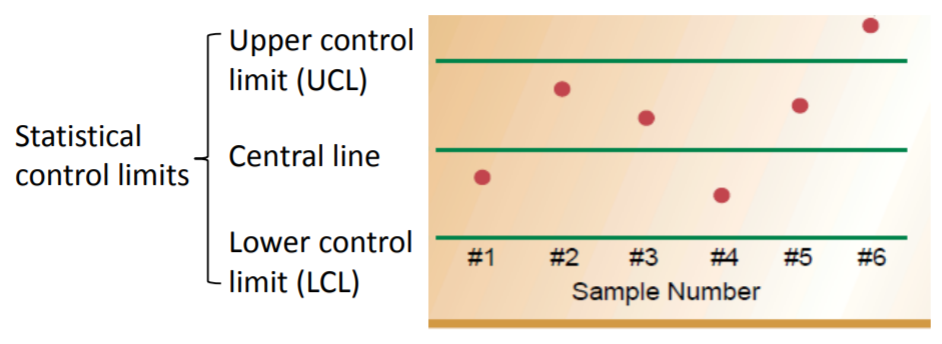
\includegraphics{D:/Documents/projects/201709.university.t6/assets/201712131943.PNG}
\caption{Statistical Control Limits}
\end{figure}

\textbf{Control charts can:}\\
- Distinguish between natural and unnatural variations - Find range of
natural variation \textbf{(this is the Control Limit)} - Examine whether
sample variation goes out of range

\begin{figure}
\centering
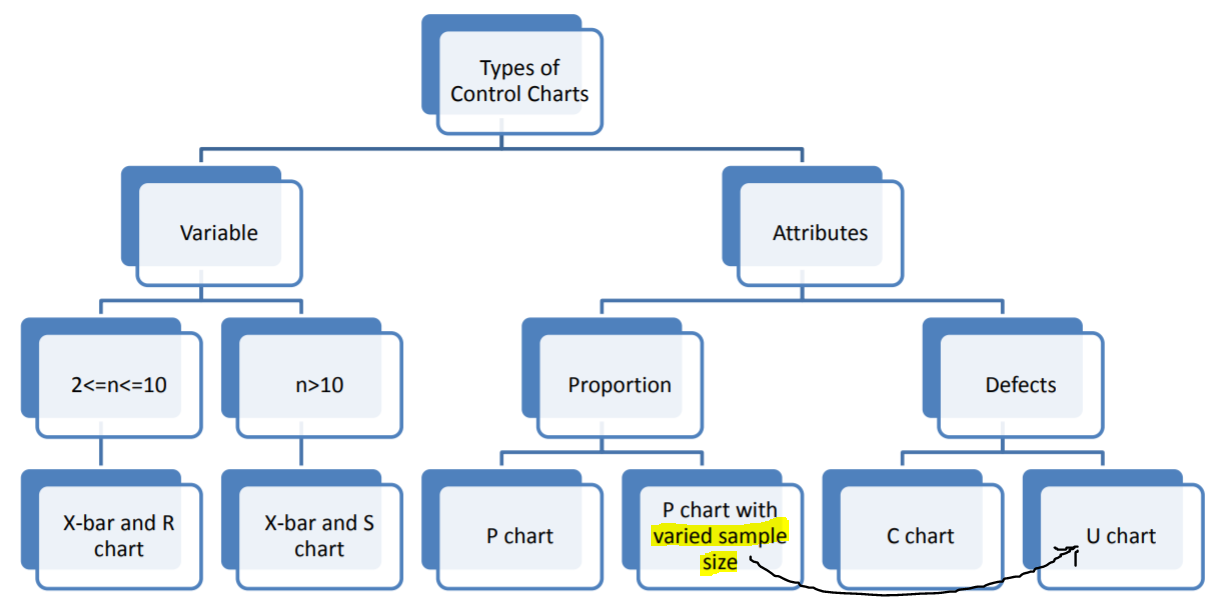
\includegraphics{D:/Documents/projects/201709.university.t6/assets/201712140309.PNG}
\caption{Control Chart Usage}
\end{figure}

\hypertarget{sources-of-variation}{%
\subsubsection{Sources of Variation}\label{sources-of-variation}}

\begin{itemize}
\tightlist
\item
  Natural Variation

  \begin{itemize}
  \tightlist
  \item
    Normal causes inherent in the process
  \item
    Can be eliminated through system improvements
  \end{itemize}
\item
  Unnatural Variation

  \begin{itemize}
  \tightlist
  \item
    Special causes
  \item
    Can also be eliminated
  \end{itemize}
\end{itemize}

Process is in control if only natural variations exist in the process

\hypertarget{control-charts-for-variables}{%
\subsubsection{Control Charts for
Variables}\label{control-charts-for-variables}}

\begin{itemize}
\tightlist
\item
  monitor characteristics with continous numerical values i.e.~height
  and weight
\item
  small sample size
\end{itemize}

\hypertarget{x-bar-control-chart}{%
\paragraph{X-Bar Control Chart}\label{x-bar-control-chart}}

\begin{itemize}
\tightlist
\item
  Examine the central tendency of the values
\item
  time-ordered plot of sample average, \(\tilde x\)
\item
  \(\tilde x\) is the average for each sample
\item
  Assumption of normality, sampling distribution follows normal
  distribution \(\bar X\sim N\left(\mu,\frac{\sigma}{\sqrt{n}}\right)\)
\item
  \(3\hat\sigma_{\bar X}=A_2\bar R\)

  \begin{itemize}
  \tightlist
  \item
    \(\bar R\): mean of sample range \emph{(refer to R Chart)}
  \item
    \(A_2\): factor depending on the sample size \emph{(check table)}
    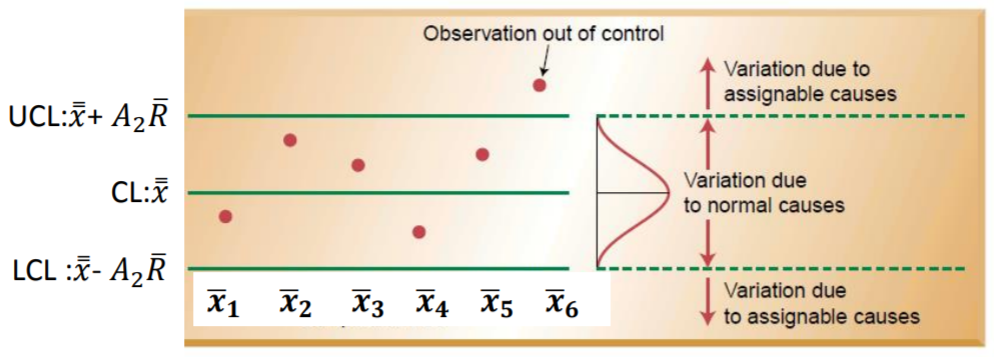
\includegraphics{D:/Documents/projects/201709.university.t6/assets/201712132356.PNG}
  \end{itemize}
\end{itemize}

\hypertarget{r-chart}{%
\paragraph{R Chart}\label{r-chart}}

\begin{itemize}
\tightlist
\item
  Examine the variations in the values
\item
  time-ordered plot of sample average \(R\)
\item
  \(R\) is the maximum range for each sample i.e.~largest value -
  smallest value
\item
  unlike X-Bar chart, the control limits for R charts are not
  symmetrical around the mean value

  \begin{itemize}
  \tightlist
  \item
    Upper Control Limit: \(D_4\bar R\)
  \item
    Lower Control Limit: \(D_3\bar R\)

    \begin{itemize}
    \tightlist
    \item
      \(D3,D4\): factor depending on the sample size \emph{(check
      table)}
    \end{itemize}
  \end{itemize}
\end{itemize}

\hypertarget{s-chart}{%
\paragraph{S Chart}\label{s-chart}}

\begin{itemize}
\tightlist
\item
  Alternative to R Chart when long-term analysis and large sample size
\item
  When used, X-Bar values for \(\sigma_{\bar X}\) changes

  \begin{itemize}
  \tightlist
  \item
    \(\sigma_{\bar X}^2=\frac{1}{n-1}\sum_{i=1}^n(x_i-\bar x)^2\)
    \emph{(unbiased estimator)}
  \end{itemize}
\item
  The S Chart has control limits:

  \begin{itemize}
  \tightlist
  \item
    Upper Control Limit: \(B_4\bar S\)
  \item
    Lower Control Limit: \(B_3\bar S\)

    \begin{itemize}
    \tightlist
    \item
      \(B3,B4\): factor depending on the sample size \emph{(check
      table)}
    \end{itemize}
  \end{itemize}
\end{itemize}

\hypertarget{control-charts-for-attributes}{%
\subsubsection{Control Charts for
Attributes}\label{control-charts-for-attributes}}

\begin{itemize}
\tightlist
\item
  monitor characteristics with discrete numerical values i.e.~number of
  defects
\item
  large sample size
\end{itemize}

\hypertarget{p-chart}{%
\paragraph{P Chart}\label{p-chart}}

\begin{itemize}
\tightlist
\item
  measure proportion of occurances i.e.~percentage of faulty items
\item
  Control Limits: \(\hat p\pm3\sigma_p\)

  \begin{itemize}
  \tightlist
  \item
    \(\sigma_p=\sqrt{\frac{\hat p(1-\hat p)}{n}}\)
  \end{itemize}
\end{itemize}

\hypertarget{c-chart}{%
\paragraph{C Chart}\label{c-chart}}

\begin{itemize}
\tightlist
\item
  measure number of occurences i.e.~number of faulty items

  \begin{itemize}
  \tightlist
  \item
    when P Chart cannot used, non-binary classification of occurences
  \end{itemize}
\item
  Control Limits: \(\max(\bar c\pm3\sqrt{\bar c}, 0)\) \emph{(lower
  limit is nonnegative)}
\end{itemize}

\hypertarget{u-chart}{%
\paragraph{U Chart}\label{u-chart}}

\begin{itemize}
\tightlist
\item
  replaces C Chart when data has varying sample sizes
\item
  also measures the number of occurences like C Chart
\item
  control limits are non-constant step functions

  \begin{itemize}
  \tightlist
  \item
    Control Limits: \(\bar u\pm3\sqrt{\frac{\bar u}{n}}\) \emph{(changes
    with n)}
  \end{itemize}
\end{itemize}

\hypertarget{zones-in-control-charts}{%
\subsubsection{Zones in Control Charts}\label{zones-in-control-charts}}

\begin{figure}
\centering
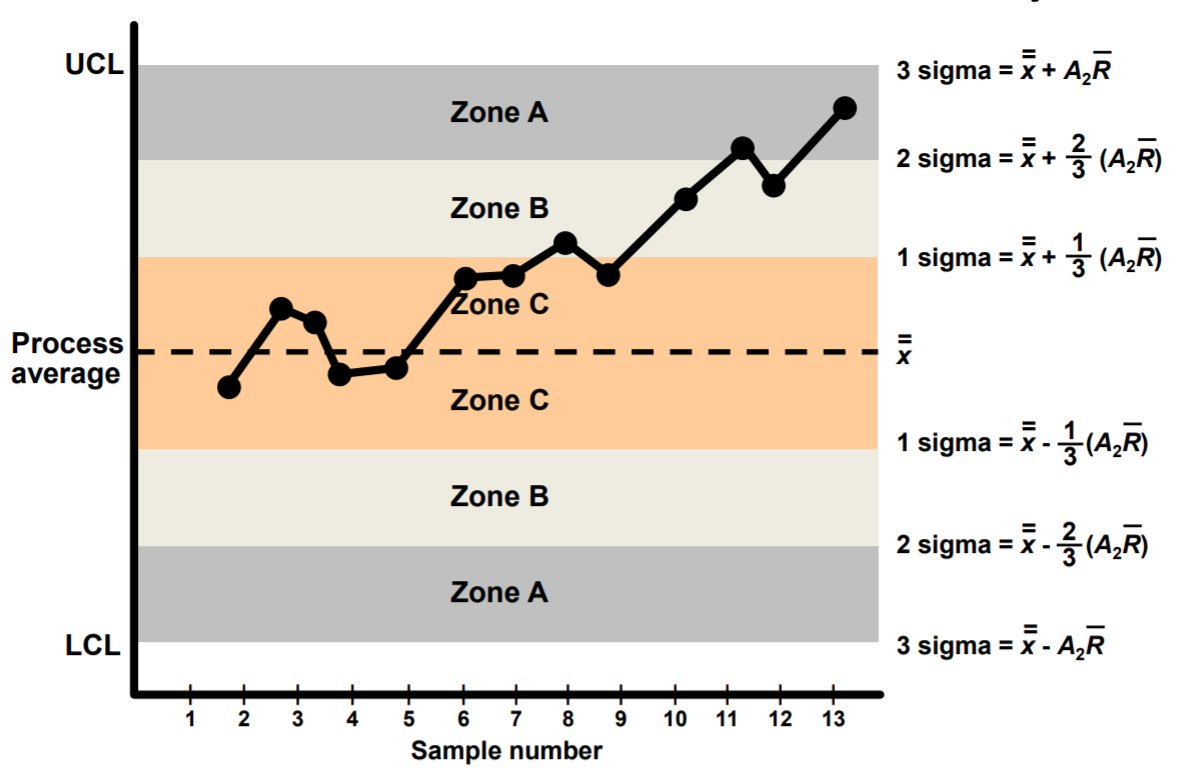
\includegraphics{D:/Documents/projects/201709.university.t6/assets/201712140325.PNG}
\caption{Control Chart Zones}
\end{figure}

\hypertarget{rules-for-out-of-control-processes}{%
\subsubsection{Rules for Out-of-Control
Processes}\label{rules-for-out-of-control-processes}}

\textbf{Process is out-of-control, if one or more of the following is
true:}\\
1. one point is above the upper control limit line or below the lower
control limit line 2. two of three consecutive points fall in zone A 3.
four of five consecutive points fall in zone A or B 4. nine consecutive
points fall on one side of the center line (above or below) 5. six
consecutive points trend upwards or downwards

\hypertarget{process-capability}{%
\subsubsection{Process Capability}\label{process-capability}}

\begin{itemize}
\tightlist
\item
  Ability of a production process to meet product specification
\item
  Product Specification \textbf{(tolerence limits)}

  \begin{itemize}
  \tightlist
  \item
    Acceptable range for quality characteristic
  \end{itemize}
\end{itemize}

\hypertarget{capability-indices}{%
\paragraph{Capability Indices}\label{capability-indices}}

\begin{itemize}
\tightlist
\item
  Process Capability Index,
  \(C_p = \frac{\text{USL} - \text{LSL}}{6\sigma}\)

  \begin{itemize}
  \tightlist
  \item
    USL: Upper Specification Limit
  \item
    LSL: Lower Specification Limit
  \item
    \(\sigma\): output standard diviation
    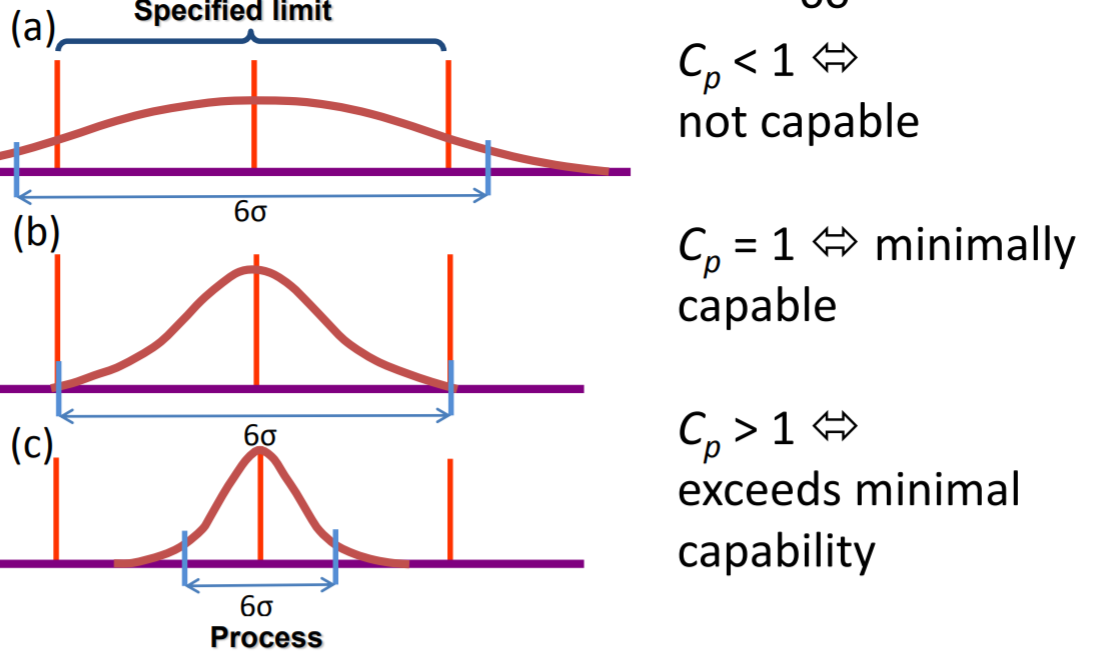
\includegraphics{D:/Documents/projects/201709.university.t6/assets/201712140412.PNG}
  \end{itemize}
\item
  One-sided Limits:

  \begin{itemize}
  \tightlist
  \item
    Upper Capability Index, \(C_{pu}=\frac{\text{USL}-\mu}{3\sigma}\)
  \item
    Lower Capability Index, \(C_{pl}=\frac{\mu-\text{LSL}}{3\sigma}\)
  \item
    Captures incapable process when process not centered
  \item
    Used when only one-side limit is given i.e.~minimum quality
  \end{itemize}
\item
  Process Capability Index, \(C_{pk}=\min\{C_{pu},C_{pl}\}\)
\end{itemize}

\begin{center}\rule{0.5\linewidth}{\linethickness}\end{center}

    \hypertarget{design-of-experiments-doe}{%
\section{Design of Experiments (DOE)}\label{design-of-experiments-doe}}

\begin{itemize}
\tightlist
\item
  Test for factors that cause variability

  \begin{itemize}
  \tightlist
  \item
    find impact of inputs on process output
  \item
    obtain estimated target levels of inputs
  \end{itemize}
\end{itemize}

\textbf{Procedure:}\\
- Conjecture \textbf{(hypothesis)} - Experiment \textbf{(perform tests)}
- Analysis \textbf{(statistical analysis of experiment data)} -
Conclusion \textbf{(accept/reject hypothesis)}

\textbf{Main challenge:} minimise noise

\textbf{Terminology:} - Input variability - Factors: controllable
variables of interest - Nuisance: variables that affect the experiment
but are not controllable or not of interest - Levels: setting/value of
factors - Response: output - Treatment: combination of levels of factors
- Experimental Unit (EU): the material being tested by the treatment
i.e.~patients or lab rats

\hypertarget{basic-experiment-design}{%
\subsection{Basic Experiment Design}\label{basic-experiment-design}}

\hypertarget{comparison-of-two-population-means}{%
\subsubsection{Comparison of Two Population
Means}\label{comparison-of-two-population-means}}

\hypertarget{two-independent-population}{%
\paragraph{Two independent
population}\label{two-independent-population}}

\begin{itemize}
\tightlist
\item
  The samples were drawn from independent populations i.e.~patients
  taking drug A or drug B
\end{itemize}

\textbf{Steps:} 1. Conditions: independent samples, \(n > 30\) 2.
Hypothesis:
\(\begin{aligned}H_0&:\mu_A-\mu_B=0\\H_a&:\mu_A-\mu_B\neq0\end{aligned}\)
3. Estimator: \(\mu_A-\mu_B\approx\bar y_A -\bar y_B\) 4. Sampling
distribution of sample mean difference:
\(\bar y_A -\bar y_B\sim N\left(\mu_A-\mu_B, \frac{\sigma_A^2}{n_A}+\frac{\sigma_B^2}{n_B}\right)\)
5. Test statistic and p-value: \(z=\frac{}{}\) 6. Accept or reject
\(H_0\)

\hypertarget{two-dependent-population}{%
\paragraph{Two dependent population}\label{two-dependent-population}}

\begin{itemize}
\tightlist
\item
  The samples were drawn from related populations i.e.~same patient
  taking drug A then drug B
\end{itemize}

\textbf{Steps:} 1. Conditions: dependent samples, \(n < 30\) 2.
Hypothesis:
\(\begin{aligned}H_0&:\mu_A-\mu_B=0\\H_a&:\mu_A-\mu_B\neq0\end{aligned}\)
3. Estimator: \(\mu_A-\mu_B\approx\bar d\) \emph{(mean of paired
difference)} 4. Sampling distribution of sample mean difference:
\(\bar d\sim t\left(\mu_A-\mu_B, \frac{\sigma_d^2}{n}\right)\) 5. Test
statistic and p-value 6. Accept or reject \(H_0\)

\hypertarget{completely-randomized-experiment}{%
\subsection{Completely Randomized
Experiment}\label{completely-randomized-experiment}}

\begin{itemize}
\tightlist
\item
  Experiment to test the effects of the primary factor
\item
  Applied when all EU are similar and only source of variation is
  primary factor
\item
  levels of primary factor assigned at random
\item
  if all treatments are equally important, balance design used
\end{itemize}

\textbf{Comparisons of Variances:} - variation within groups:
\(\sigma^2\) estimated by the variance of each sample, \(s^2_W\) -
variation between groups: if means are equal, \(\sigma^2\) can be
estimated by \(s^2_B\), the product of sample size and the sample
variance of sample means
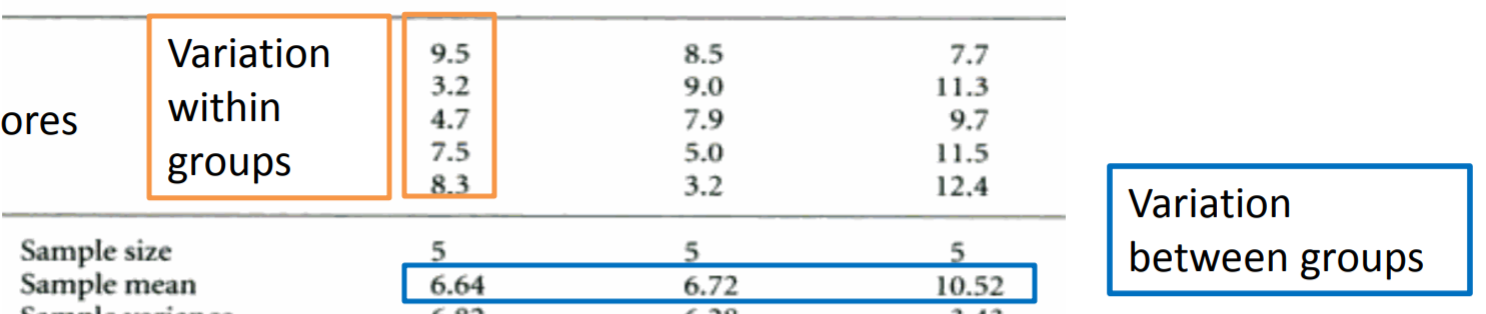
\includegraphics{D:/Documents/projects/201709.university.t6/assets/201712140902.PNG}
\emph{(both should be equal if means are equal)}

\textbf{Hypothesis Testing:} 1. Hypothesis:
\(\begin{aligned}H_0&:\mu_1=\mu_2=\mu_3\\H_a&:\text{not all population means are the same}\end{aligned}\)
2. Estimator: \(\frac{s_B^2}{s_W^2}\) - close to 1 in normal cases -
follows F-distribution if between 2-12 degrees of freedom 3. Test
statistic and p-value: \(\frac{s_B^2}{s_W^2}\) 4. Accept or reject
\(H_0\)

\textbf{cases} - balanced (\(n_i=n_j, \forall i,j\)) - unbalanced
(one-way anova)\\
\(\frac{s^2_B}{s_W^2}=\frac{\sum_{i=1}^kn_i(\bar y_i-\bar y)^2/(k-1)}{\sum_{i=1}^k\sum_{j=1}^{n_i}(y_{ij}-\bar y_i)^2/(N-k)}=\frac{\text{SSB: Sum of square between groups}/(k-1)}{\text{SSW: Sum of square within groups}/(N-k)}=\frac{\text{MSB}}{\text{MSW}}\)

\textbf{terminologies} - SS: sum of squares of observantion from the
mean - MS: mean squares = SS/Degrees of freedom

\hypertarget{randomized-complete-block-experiment}{%
\subsection{Randomized Complete Block
Experiment}\label{randomized-complete-block-experiment}}

\begin{itemize}
\tightlist
\item
  when EU are non homogenous, we need to group the similar EU into
  blocks
\item
  Experiment to test the effects of the primary factor while one or more
  nuisance factors are known and controllable
\item
  Similar nuisance factors are in same block

  \begin{itemize}
  \tightlist
  \item
    each treatment is assigned to every block
  \item
    with each treatment randomly assigned within the block
  \end{itemize}
\item
  use two-way ANOVA
  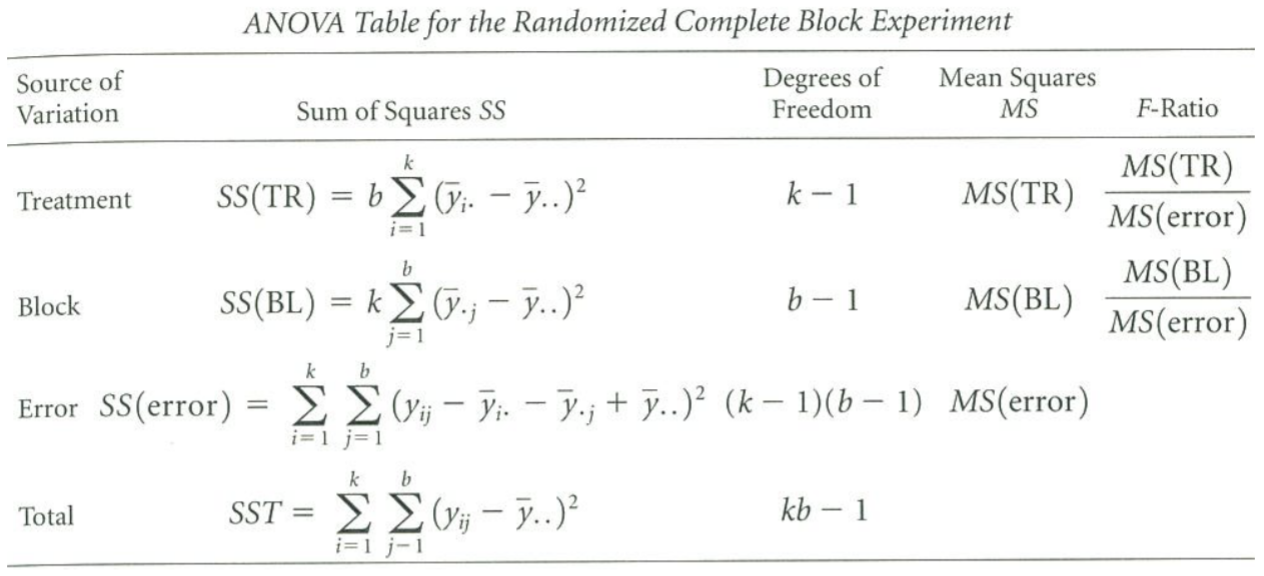
\includegraphics{D:/Documents/projects/201709.university.t6/assets/201712140938.PNG}
\end{itemize}

    \hypertarget{factorial-design}{%
\subsection{Factorial Design}\label{factorial-design}}

\begin{itemize}
\tightlist
\item
  Studies the effect of two or more factors

  \begin{itemize}
  \tightlist
  \item
    Main effect: how the response changes with each factor
  \item
    Interaction effect: how one factor affects the effectiveness of
    another factor
  \end{itemize}
\end{itemize}

\hypertarget{calculation-of-effects}{%
\subsubsection{Calculation of Effects}\label{calculation-of-effects}}

\begin{itemize}
\tightlist
\item
  Main Effect: \(A=\bar y_{A^+}-\bar y_{A^-}\)
\item
  Interaction Effect:
  \(AB=\frac{1}{2}[(y_{A^+B^+}-y_{A^-B^+})-(y_{A^+B^-}-y_{A^-B^-})]\)
\end{itemize}

\hypertarget{factorial-anova}{%
\subsubsection{Factorial ANOVA}\label{factorial-anova}}

\begin{itemize}
\tightlist
\item
  ANOVA with more than two factors with more than one level
\item
  Notation: 2x3x4 ANOVA, 3 factors with 2,3,4 levels respectively
\end{itemize}

\begin{figure}
\centering
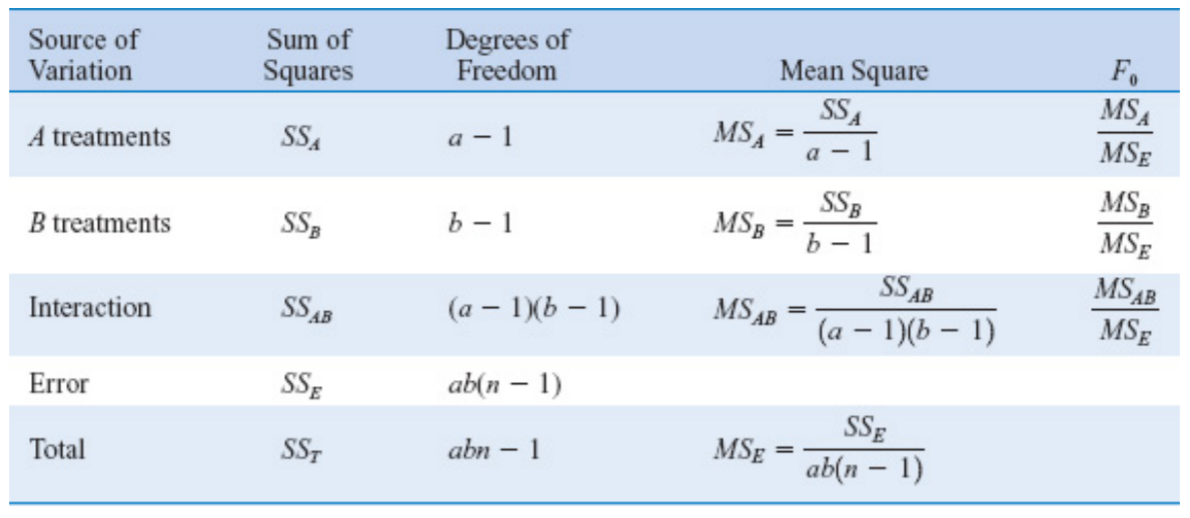
\includegraphics{D:/Documents/projects/201709.university.t6/assets/201712141333.PNG}
\caption{two factor ANOVA}
\end{figure}

\begin{center}\rule{0.5\linewidth}{\linethickness}\end{center}

    \hypertarget{system-reliability}{%
\section{System Reliability}\label{system-reliability}}

\hypertarget{time-to-failure}{%
\subsection{Time-to-Failure}\label{time-to-failure}}

\begin{itemize}
\tightlist
\item
  Mean Time to Failure, \(\text{MTTF} = \int_0^\infty tf(t)\ dt\)

  \begin{itemize}
  \tightlist
  \item
    \(f(t)\): probability density function
  \item
    \(F(t)\): cumalative distribution function
  \end{itemize}
\item
  Reliability:

  \begin{itemize}
  \tightlist
  \item
    Discrete: \(R(t)=1-F(t-1)\)
  \item
    Continuous: \(R(t)=1-F(t)\)
  \item
    \(\text{MTTF}=\int_0^\infty R(t)\ dt\)
  \end{itemize}
\end{itemize}

\hypertarget{failure-rate}{%
\subsection{Failure Rate}\label{failure-rate}}

\begin{itemize}
\item
  probability of failure in the next unit time
\item
  \(\lambda(t)=\frac{f(t)}{R(t)}\)
\item
  constant failure rate:

  \begin{itemize}
  \tightlist
  \item
    \(\lambda(t)=\frac{f(t)}{R(t)}=\lambda\)
  \item
    \(\text{MTTF}=\frac{1}{\lambda}\)
  \end{itemize}
\end{itemize}

\hypertarget{life-cycle-curve}{%
\subsection{Life Cycle Curve}\label{life-cycle-curve}}

\begin{itemize}
\tightlist
\item
  failure rate over time
\item
  Normal scenario: Bathtub Curve
  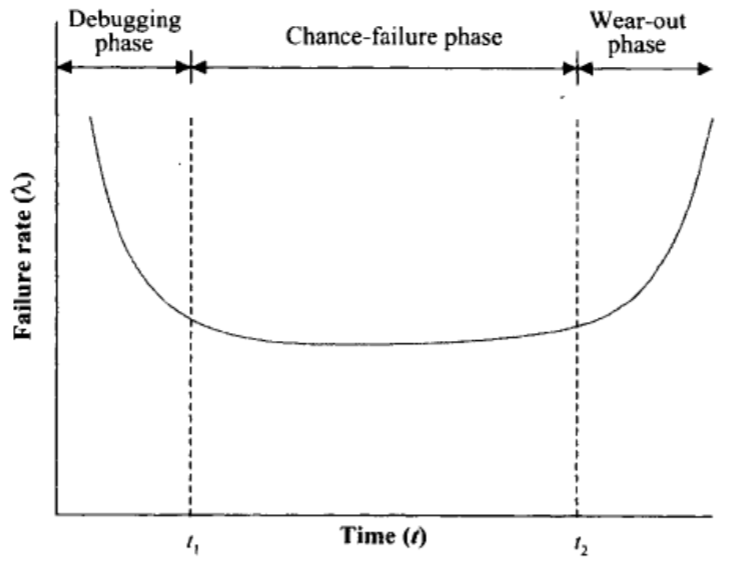
\includegraphics{D:/Documents/projects/201709.university.t6/assets/201712141351.PNG}
\end{itemize}

\hypertarget{system-reliability-1}{%
\subsection{System Reliability}\label{system-reliability-1}}

\hypertarget{in-series}{%
\subsubsection{In series}\label{in-series}}

\begin{itemize}
\tightlist
\item
  \(R_s=R_1\times R_2\times...\times R_n\)
\item
  For Exponential model

  \begin{itemize}
  \tightlist
  \item
    \(R_i=e^{-\lambda_i t}\)
  \item
    \(R_s = e^{-\sum_{i=1}^n\lambda_it}\)
  \item
    \(\lambda_s = \sum_{i=1}^n\lambda_i\)
  \item
    \(\text{MTTF}=\frac{1}{\sum_{i=1}^n\lambda_i}\)
  \end{itemize}
\end{itemize}

\hypertarget{in-parallel}{%
\subsubsection{In Parallel}\label{in-parallel}}

\begin{itemize}
\tightlist
\item
  System failure probability, \(F_s=\prod_{i=1}^n(1-R_i)\)
\item
  \(R_s=1-F= 1-\prod_{i=1}^n(1-R_i)\)
\item
  For exponential model

  \begin{itemize}
  \tightlist
  \item
    \(R_i=e^{-\lambda_i t}\)
  \item
    \(R_s=1-\prod_{i=1}^n(1-e^{-\lambda_it})\)
  \item
    \(\text{MTTF}=\int_0^nR_s\ dt\)
  \item
    if all failure rate the same,
    \(\text{MTTF}=\frac{1}{\lambda}\times(1+\frac{1}{2}+\frac{1}{3}+...+\frac{1}{n})\)
  \end{itemize}
\end{itemize}


    % Add a bibliography block to the postdoc
    
    
    
    \end{document}
